\documentclass{article}
\usepackage{fullpage}
\usepackage{wasysym}
\usepackage{verbatim}
\usepackage[usenames,dvipsnames]{color}
\usepackage{graphicx}
\usepackage[bookmarks=false]{hyperref}
\usepackage[colour]{circus}
\usepackage{hijac}
\usepackage{accs_spec}

\hypersetup{colorlinks=true,linkcolor=black,citecolor=red,urlcolor=blue}

\title{Abstract {\Circus} Model for the Cruise Controller}

\author{Frank Zeyda}

\begin{document}

\maketitle

\tableofcontents

\newpage

%%%%%%%%%%%%%%%%%%%%%%%%%%%%%%%%%%%%%%%%%%%%%%%%%%%%%%%%%%%%%%%%%%%%%%%%%%%%%%%%
%                                 Requirements                                 %
%%%%%%%%%%%%%%%%%%%%%%%%%%%%%%%%%%%%%%%%%%%%%%%%%%%%%%%%%%%%%%%%%%%%%%%%%%%%%%%%

%\section{Requirements}

%\newpage

%%%%%%%%%%%%%%%%%%%%%%%%%%%%%%%%%%%%%%%%%%%%%%%%%%%%%%%%%%%%%%%%%%%%%%%%%%%%%%%%
%                                 Preliminaries                                %
%%%%%%%%%%%%%%%%%%%%%%%%%%%%%%%%%%%%%%%%%%%%%%%%%%%%%%%%%%%%%%%%%%%%%%%%%%%%%%%%

%\section{Preliminaries}

%Definitions of auxiliary Z types, constants and functions.
%
%\input{Preliminaries.circus}

%\newpage

%%%%%%%%%%%%%%%%%%%%%%%%%%%%%%%%%%%%%%%%%%%%%%%%%%%%%%%%%%%%%%%%%%%%%%%%%%%%%%%%
%                               Global Constants                               %
%%%%%%%%%%%%%%%%%%%%%%%%%%%%%%%%%%%%%%%%%%%%%%%%%%%%%%%%%%%%%%%%%%%%%%%%%%%%%%%%

\section{Global Constants}

In this section we define a few global constants that are used later on in some of the calculations.
%
\input{GlobalConstants.circus}

\newpage

%%%%%%%%%%%%%%%%%%%%%%%%%%%%%%%%%%%%%%%%%%%%%%%%%%%%%%%%%%%%%%%%%%%%%%%%%%%%%%%%
%                             Channels for Sensors                             %
%%%%%%%%%%%%%%%%%%%%%%%%%%%%%%%%%%%%%%%%%%%%%%%%%%%%%%%%%%%%%%%%%%%%%%%%%%%%%%%%

\section{Channels for Sensors}

In this section we define channels for sensor events.
%
\input{SensorChannels.circus}

\newpage

%%%%%%%%%%%%%%%%%%%%%%%%%%%%%%%%%%%%%%%%%%%%%%%%%%%%%%%%%%%%%%%%%%%%%%%%%%%%%%%%
%                            Channels for Actuators                            %
%%%%%%%%%%%%%%%%%%%%%%%%%%%%%%%%%%%%%%%%%%%%%%%%%%%%%%%%%%%%%%%%%%%%%%%%%%%%%%%%

\section{Channels for Actuators}

In this section we define the channel for actuator event.
%
\input{ActuatorChannels.circus}

%\newpage

%%%%%%%%%%%%%%%%%%%%%%%%%%%%%%%%%%%%%%%%%%%%%%%%%%%%%%%%%%%%%%%%%%%%%%%%%%%%%%%%
%                              Channels for Times                              %
%%%%%%%%%%%%%%%%%%%%%%%%%%%%%%%%%%%%%%%%%%%%%%%%%%%%%%%%%%%%%%%%%%%%%%%%%%%%%%%%

%\input{TimerChannels.circus}

\newpage

%%%%%%%%%%%%%%%%%%%%%%%%%%%%%%%%%%%%%%%%%%%%%%%%%%%%%%%%%%%%%%%%%%%%%%%%%%%%%%%%
%                               Internal Channels                              %
%%%%%%%%%%%%%%%%%%%%%%%%%%%%%%%%%%%%%%%%%%%%%%%%%%%%%%%%%%%%%%%%%%%%%%%%%%%%%%%%

\section{Specification Events}

The channels in this section are used solely for specification purposes and are thus concealed in the top-level model of the cruise controller. This also makes the respective events urgent and therefore we do not need to impose deadlines of any sort on them. We require them for interaction of the specification components.
%
\input{InternalChannels.circus}

\newpage

%%%%%%%%%%%%%%%%%%%%%%%%%%%%%%%%%%%%%%%%%%%%%%%%%%%%%%%%%%%%%%%%%%%%%%%%%%%%%%%%
%                                Model Analysis                                %
%%%%%%%%%%%%%%%%%%%%%%%%%%%%%%%%%%%%%%%%%%%%%%%%%%%%%%%%%%%%%%%%%%%%%%%%%%%%%%%%

%%%%%%%%%%%%%%%%%%%%%%%%%%%%%%%%%%%%%%%%%%%%%%%%%%%%%%%%%%%%%%%%%%%%%%%%%%%%%%%%%
%                                Model Analysis                                %
%%%%%%%%%%%%%%%%%%%%%%%%%%%%%%%%%%%%%%%%%%%%%%%%%%%%%%%%%%%%%%%%%%%%%%%%%%%%%%%%

\section{Model Analysis}

\subsection{State Machine}

Part of the behavioural requirements of the cruise controller are captured by a state transition diagram~\cite{Wel04}. In this section we discuss its impact on the formal model, and the assumptions we make about its semantics.

\paragraph{Semantics of Transitions}

In the original diagram in~\cite{Wel04}, which is based on the cruise controller case study in~\cite{HP87}, we do not have an outgoing transition for every event from every state. In one or two cases this was an erroneous omission, but there are also cases where it may be viewed as intentional; specifically with regards to the lever events which it disallows from certain states. For instance, we may prohibit the $lever~.~activate$ event from a state where we are braking or running in low gear.

The questions is hence what does it \emph{mean} if there is no outgoing transition for a particular event in a given state. The simple answer is that such an event cannot occur. Thus we either make an assumption that the environment will `behave' and never engage in such an event, or otherwise the interface, namely the hardware, prohibits it by some physical mechanism. A locking contraption, for example, prevent us from putting the lever into the activate position if we are not running in top gear.

A better view is that events in the specification do not actually correspond to physical happenings, but already involve some level of interpretation by the hardware and software. For one, it might not be possible to stop the brake pedal from being pressed, or to stop the command lever from being operated. And besides it should not fall to some physical mechanism in the lever to determine whether we can enter cruise mode or not~(such a mechanism may be a critical point of failure). Hence, I believe a more coherent view is:
%
\begin{center}
\bluebox{Events generally do not correspond to physical happenings but detectable interrupts.}
\end{center}
%
This means that we do not necessarily assume there is something physical that stops the user from switching the position of the lever or pressing the brake pedal at the same time. Instead, we assume that those events give rise to interrupts, and the interrupts correspond to interactions with the environment where there are first observed from the program's point of view. The underlying physical events causing the interrupts are a different issue, and we may model the relationship between physical events and interrupts, or we may not. If we do, different approaches are conceivable; however, in the cruise controller we decide not to.

This means that in the cruise controller, effectively, the program can `prohibit' events by disabling interrupts. It does not necessarily mean that we cannot physically press the brake pedal or operate the lever at certain points in time; if we do, there could be different resolutions such as ignoring the event or buffering it, but we choose it is outside the scope of our program model to formalise this relationship.
%
\begin{center}
\bluebox{Physical happenings are an aspect of the model that we may consider, or may not consider.}
\end{center}
%
An implication of this is that when we subsequently impose requirements on the inter-arrival time of aperiodic events, this does not actually relate to the physical events but the \emph{mechanism that responds to physical events}.

Such mechanism may de-bounce the contact of a switch, limit the frequency of events in a certain interval, or ensure that events have a minimal inter-arrival time. Indeed, no software system will be able to respond in a scenario where events can take place in arbitrary short succession and density. If we did model the relationship between physical happenings and interrupts, there would need to be requirements that physical happenings cannot occur in arbitrary short succession, or if they do they may be ignored by the application. But this is not a problem, just a level of detail that we chose not to treat in the program model.

\paragraph{Behavioural Requirements}

The state machine fulfils two purposes. First, it restricts interaction of the environment with the program. For instance, if we are running in a low gear and the driver tries to put the lever into the activate position, nothing should happen~(or alternatively it may not even be possible). In an SCJ implementation this effectively requires to take control of interrupts within the handler methods. The implementation must also ensure perfect synchronity:~that is no event (interrupt) can occur before the transition and action according to some earlier event has been carried out, whatever this means.

But even identifying the actions that correspond to the transitions~(we can think of them as internal outputs) we still have the two design alternatives: should lever interrupts be possible all the time? The cruise controller implementation in~\cite{Wel04} does not restrict interrupts, and hence suggests an abstract model where we can operate the lever even in a state where activation does not succeed. Here, simply nothing happens in the system. In accordance, I present two revised models for the cruise controller state transition diagram:~one that restricts interaction via lever event~(Appendix~\ref{apx:asm1}) and one where lever events can always occur~(Appendix~\ref{apx:asm2}). My conjecture after talking to Andy Wellings is that both models are implementable and make sense. We could even envisage a third model where the actions are factored out into a separate state diagram, however I decided that this separation does not aid the understanding of the system.
%
\begin{center}
\bluebox{The purpose of state diagrams is twofold:~restrict user interaction and specify associated actions.}
\end{center}
%
We may also conclude that we can capture such diagrams by a particular abstract modelling pattern in {\Circus} as well as a particular implementation that may need to take charge of enabling / disabling interrupts. It is clear, however, that the diagram captures and essential part of the behavioural requirements, and cannot be ignored in terms of providing a model for the entire cruise control system. We could, of course, express it as a process in different ways, namely by changing the representation of the state. However, my personal take is that we should allow the requirements engineer to use whatever notation seems most familiar and easy to understand, and rather shift the problem in terms of giving a semantics to that notation~(here some state chart formalism) in terms of our unifying {\Circus} notation.

\paragraph{Timing Requirements}

Where no timing information is giving in a state transition diagram, one typically assume that transitions are \emph{instantaneous}, hence take not time. I believe that in our interpretation of the diagram we ought to relax this view:~rather than saying something explicit about time, we acknowledge that we simply do not have information how much time particular transitions take. The reasons for this are:
%
\begin{enumerate}
  \item Time should be a separate concern from the behavioural perspective of the diagram.

  \item In a real system it may be too strong to assume that transitions are instantaneous. A program may take some time to record them in suitable data objects, and knowledge of that time may be a crucial factor in reasoning about the correctness of the SCJ program.
\end{enumerate}
%
In summary, the only invariant requirement we make is that of perfect synchroniety, namely that events can only take place when transitions have been fully committed and the underlying actions have been performed. Time, at the level of the state diagram, is only an issue as far as the diagram is \emph{implementable}. And for this we identify a certain amount of time, captured by non-deterministic waits in the abstract model, that enables an implementation to carry out the internal data operations that correspond to the state changes.

On the other hand, if some (or all) actions of transitions are performed \emph{synchronously} rather than \emph{asynchronously}, and hence we anticipate they take a specific amount of time, this information needs to be added to the model. Here, we do not examine in detail how this may be done. An obvious possibility is to each annotate transition with a minimal time or alternatively time interval that reflects the time the actual system (program) may take to carry out the underlying action.

In the cruise controller, the actions of transitions are all asynchronous and considered as virtually instantaneous. In the model, they correspond to internal events that request activation ($activate$), deactivation ($deactivate$) and acceleration ($accelerate$) mode. Thus, the only time we have to account for is effectively to allow the program to record the state transitions.
%
\begin{center}
\bluebox{Actions associated with transitions in the cruise controller diagram are executed asynchronously.}
\end{center}

\paragraph{Conclusions}

State charts seem to be a formalism that engineers are familiar with. Hence, it is worth to investigate if we can integrate them with our general approach of specifying systems in {\Circus}. Clearly, there are some semantic issues that need to be addressed, and the objective here was at least to shed some light into them. Eventually, we are seeking for a notation that will hide the details of the {\Circus} model, and it is conceivable that such a notation will borrow from different languages and notations used for functional, behavioural and timing requirements by defining a semantics for them in terms of {\Circus} while ensuring non-interference of modelling concerns. The account here is mostly given so that the {\Circus} models presented in the next section can be traced back to the diagrams in the appendix.


%\newpage

%%%%%%%%%%%%%%%%%%%%%%%%%%%%%%%%%%%%%%%%%%%%%%%%%%%%%%%%%%%%%%%%%%%%%%%%%%%%%%%%
%                                Abstract Model                                %
%%%%%%%%%%%%%%%%%%%%%%%%%%%%%%%%%%%%%%%%%%%%%%%%%%%%%%%%%%%%%%%%%%%%%%%%%%%%%%%%

\section{Abstract Model}

In this section we present the abstract model of the cruise controller. It factors into four parallel components that capture the semantics of the state diagram, speed monitor, throttle controller, and timing requirements.

%%%%%%%%%%%%%%%%%%%%%%%%%%%%%%%%%%%%%%%%%%%%%%%%%%%%%%%%%%%%%%%%%%%%%%%%%%%%%%%%

\subsection{State Machine}

In this section we specify the process that corresponds to the state transition diagram.
%
\input{StateMachine.circus}

%%%%%%%%%%%%%%%%%%%%%%%%%%%%%%%%%%%%%%%%%%%%%%%%%%%%%%%%%%%%%%%%%%%%%%%%%%%%%%%%

\subsection{Interarrival Times}

In this section we specify inter-arrival times of events.
%
\input{InterArrivalTimes.circus}

\newpage

%%%%%%%%%%%%%%%%%%%%%%%%%%%%%%%%%%%%%%%%%%%%%%%%%%%%%%%%%%%%%%%%%%%%%%%%%%%%%%%%

\subsection{Speed Monitor}

In this section we specify the behaviour of the abstract component that monitors the speed.
%
\input{SpeedMonitor.circus}

%%%%%%%%%%%%%%%%%%%%%%%%%%%%%%%%%%%%%%%%%%%%%%%%%%%%%%%%%%%%%%%%%%%%%%%%%%%%%%%%

\subsection{Throttle Controller}

In this section we specify the behaviour of the abstract component that controls the throttle.
%
\input{ThrottleControl.circus}

\newpage

%%%%%%%%%%%%%%%%%%%%%%%%%%%%%%%%%%%%%%%%%%%%%%%%%%%%%%%%%%%%%%%%%%%%%%%%%%%%%%%%

\subsection{Timing Requirements}

In this section we specify various timing requirements of the cruise control system. They are on one hand response times when the system must acquire (or release) control of the throttle, and on another specify the maximum delay between two $set\_voltage$ events when cruising or accelerating. Informal descriptions of the requirements imposed by particular process actions are included in Table~\ref{tab:informaltimingreq}.
%
\input{ThrottleTiming.circus}

\begin{table}
\centering
\begin{tabular}{c c}
  \textbf{Process Action} & \textbf{Informal Description}\\
\hline
\hline
   $TReq1$ &
   \parbox{0.6\textwidth}{
   \smallskip
   When the user requests that cruise mode should be activated, the system should be in control of the speed within $activate\_deadline$ seconds.
   \smallskip}\\
\hline
   $TReq2$ &
   \parbox{0.6\textwidth}{
   \smallskip
   When the user requests that cruise mode should be deactivated, the system should give up control of the speed within $deactivate\_deadline$ seconds.
   \smallskip}\\
\hline
   $TReq3$ &
   \parbox{0.6\textwidth}{
   \smallskip
   When the user requests that acceleration mode should be activated, the system should be in control of the speed and accelerating within $start\_acceleration$ seconds.
   \smallskip}\\
\hline
   $TReq4$ &
   \parbox{0.6\textwidth}{
   \smallskip
   When the user requests that acceleration mode should be deactivated, the system should be in control of the speed and cruising within $stop\_acceleration$ seconds.
   \smallskip}\\
\hline
   $TReq5$ &
   \parbox{0.6\textwidth}{
   \smallskip
   When the user requests that cruise mode should be resumed, the system should be in control of the speed within $resume\_deadline$ seconds.
   \smallskip}\\
\hline
   $TReq6$ &
   \parbox{0.6\textwidth}{
   \smallskip
   Writes of the throttle voltage must occur with a certain frequency while the system is in control. We thus constrain the maximum delay between two writes to be $set\_voltage\_max\_delay$.
   \smallskip}\\
\hline
   $TReqWriteVoltage$ &
   \parbox{0.6\textwidth}{
   \smallskip
   This requirement is an artifact of the model. It states that the $set\_voltage$ event must occur immediately after $write\_voltage$. It justifies the use of $write\_voltage$ rather than $set\_voltage$ in the other timing requirements.
   \smallskip}\\
\hline
\end{tabular}
\caption{Informal description of the timing requirements for the throttle.}
\label{tab:informaltimingreq}
\end{table}

%\newpage

%%%%%%%%%%%%%%%%%%%%%%%%%%%%%%%%%%%%%%%%%%%%%%%%%%%%%%%%%%%%%%%%%%%%%%%%%%%%%%%%

\subsection{Complete System}

In this section we specify the top-level system model.
%
\input{System.circus}

\newpage

%%%%%%%%%%%%%%%%%%%%%%%%%%%%%%%%%%%%%%%%%%%%%%%%%%%%%%%%%%%%%%%%%%%%%%%%%%%%%%%%
%                                Previous Model                                %
%%%%%%%%%%%%%%%%%%%%%%%%%%%%%%%%%%%%%%%%%%%%%%%%%%%%%%%%%%%%%%%%%%%%%%%%%%%%%%%%

%\section{Previous Model}

%The previous centralised process for the abstract model of the cruise controller system is given below.
%
%\input{PreviousModel.circus}

%\newpage

%%%%%%%%%%%%%%%%%%%%%%%%%%%%%%%%%%%%%%%%%%%%%%%%%%%%%%%%%%%%%%%%%%%%%%%%%%%%%%%%
%                                 Bibliography                                 %
%%%%%%%%%%%%%%%%%%%%%%%%%%%%%%%%%%%%%%%%%%%%%%%%%%%%%%%%%%%%%%%%%%%%%%%%%%%%%%%%

\bibliographystyle{plain}

\bibliography{accs_spec}

%%%%%%%%%%%%%%%%%%%%%%%%%%%%%%%%%%%%%%%%%%%%%%%%%%%%%%%%%%%%%%%%%%%%%%%%%%%%%%%%
%                                   Appendix                                   %
%%%%%%%%%%%%%%%%%%%%%%%%%%%%%%%%%%%%%%%%%%%%%%%%%%%%%%%%%%%%%%%%%%%%%%%%%%%%%%%%

\appendix

\section{Appendix}
\label{apx:asms}

\subsection{State Diagram 1:~Blocking Version}
\label{apx:asm1}

\begin{center}
\vspace{1ex}
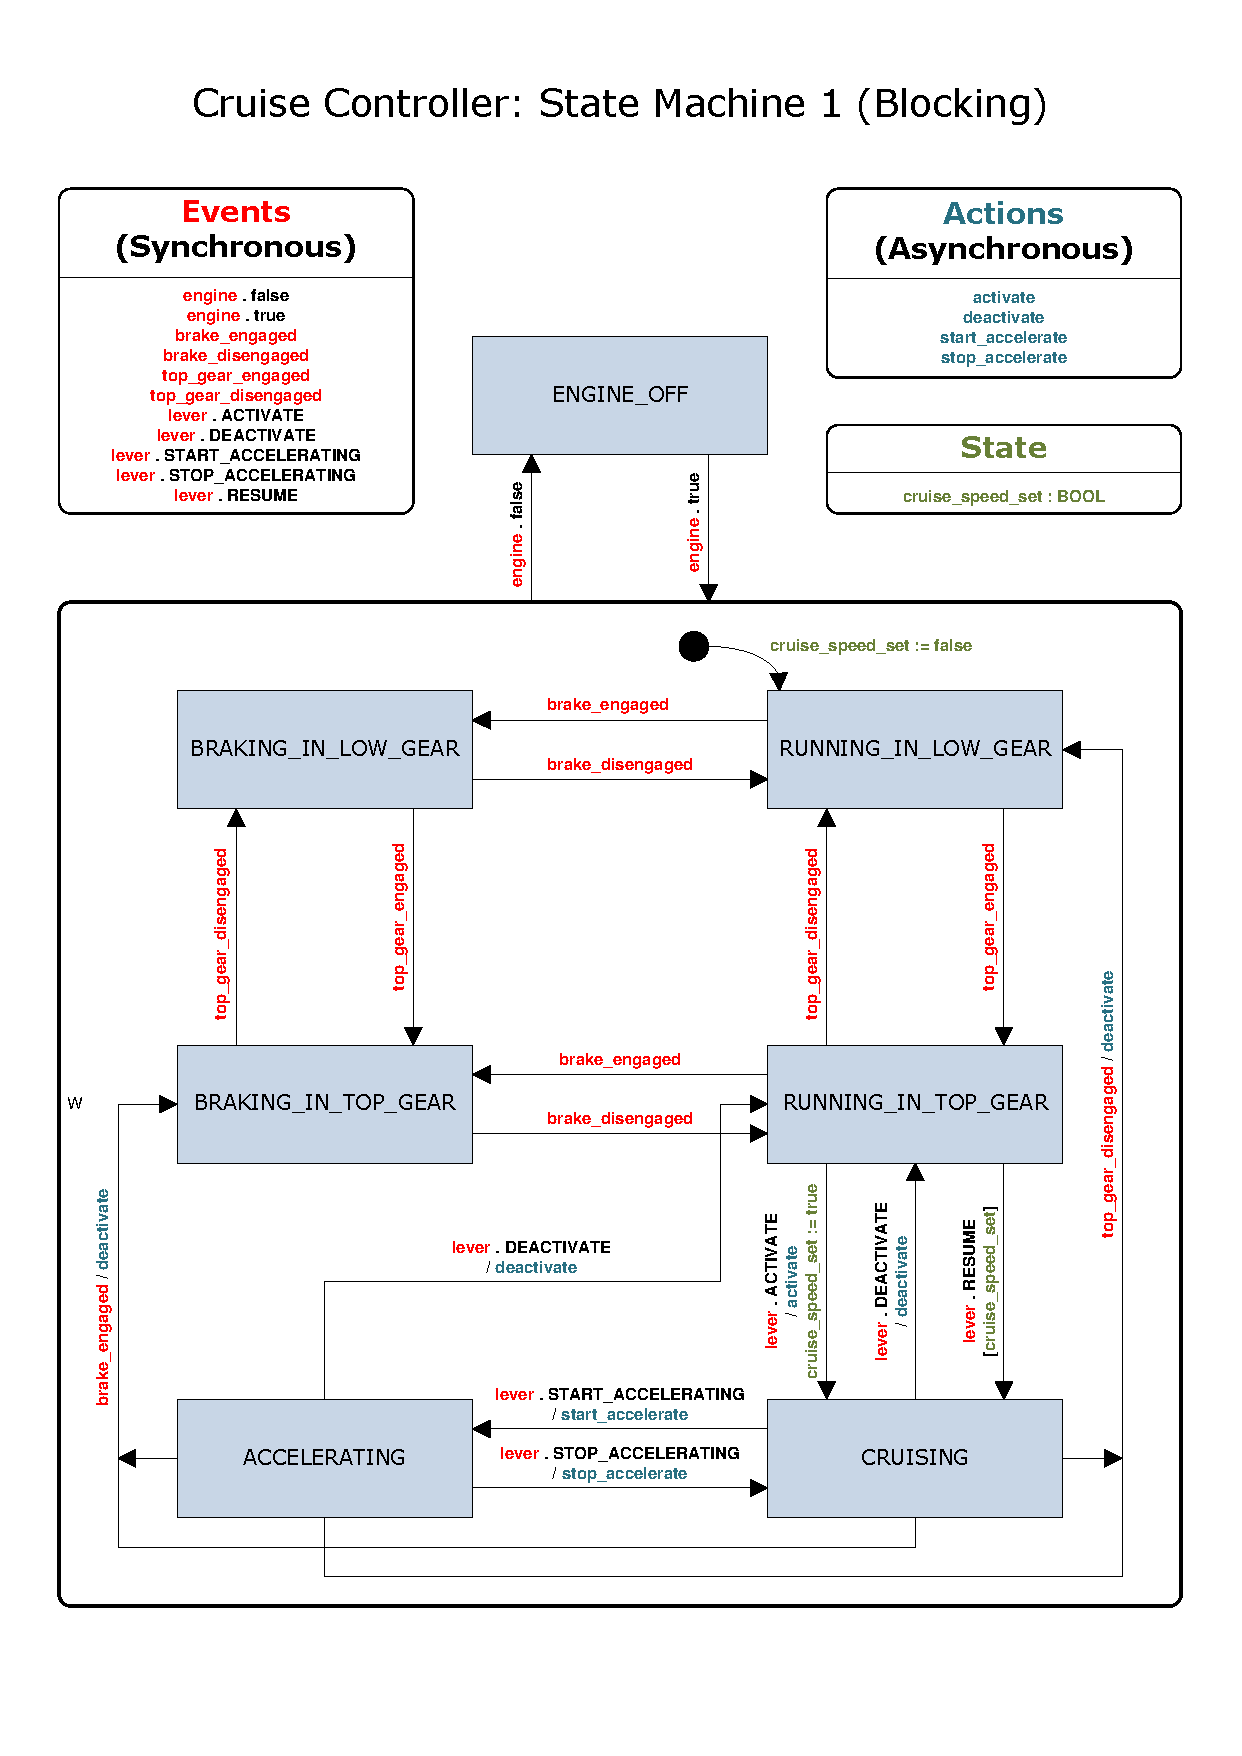
\includegraphics[scale=0.77,trim=20 65 20 80,clip]{CruiseControllerAMS1.pdf}
\end{center}

\nid The blocking version of the state machine is closest to the state machine model presented in \cite{Wel04}. However, its implementation is more complex since it requires a more subtle control of interrupts.

\subsection{State Diagram 2:~Nonblocking Version}
\label{apx:asm2}

The nonblocking version of the state machine is the model that was actually implemented in \cite{Wel04}.
%
\begin{center}
\vspace{1ex}
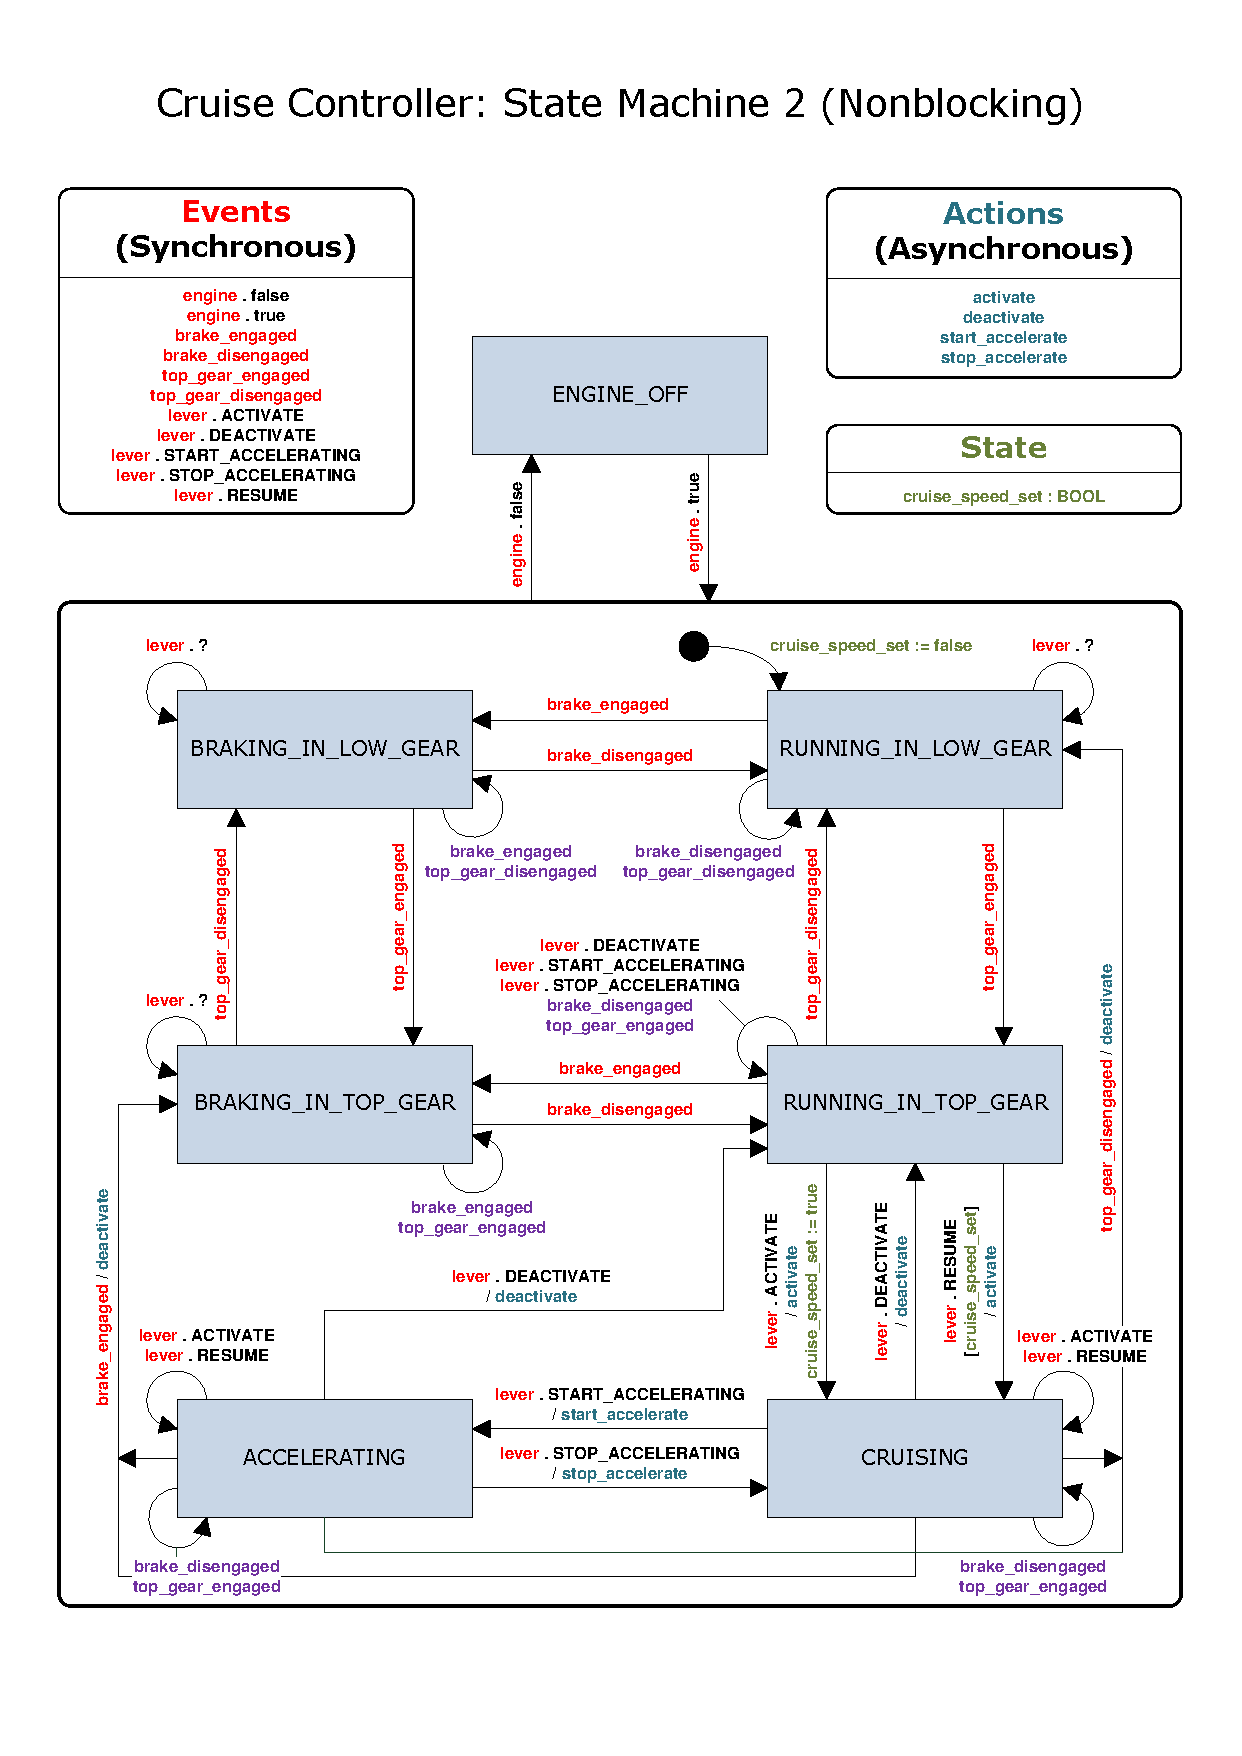
\includegraphics[scale=0.77,trim=20 65 20 80,clip]{CruiseControllerAMS2.pdf}
\end{center}
%
\nid In \purple{purple} we highlight events that we do not expect to take place. Nonetheless we require the application to deal with them in a way that they are ignored. Important is here that even though we think of those events constraining the environment, we do not diverge if the environment does not `behave'.

\end{document}
